%+================+
%| DOCUMENT SETUP |
%+================+

% Set document class
\documentclass[xcolor=dvipsnames,11pt,paper=a4paper]{report}

% Include packages
% Encryption and spelling
\usepackage[utf8]{inputenc}
\usepackage[T1]{fontenc}
\usepackage[ngerman]{babel}

% Font type
%\usepackage{DejaVuSansMono}	% Replaces original typewriter font
\usepackage{kpfonts}

% Drawings and color
\usepackage{graphicx}
\usepackage{tikz}
\usepackage{xcolor}

% Formatting packages
\usepackage[top=1in, right=1.25in, bottom=1in, left=1.25in]{geometry}	% For page layout. 1in/1.25in is default in Office Word
\usepackage{wrapfig}		% Text wrapped around images
\usepackage{tocloft}		% Better Table of Contents etc.
\usepackage{listings}	% For code listings
\usepackage{fancyhdr}	% For footer/header settings
\usepackage{chngcntr}	% Stops resetting footnote counter
\usepackage[hidelinks=true]{hyperref}	% For links
\usepackage{titlesec}	% For better chapter style
\usepackage{enumitem}	% For better enumerate/itemize style
\usepackage{float}			% For fixed image positioning
% \usepackage{svg} % For SVG images
%\usepackage{pythonhighlight}
\renewcommand*{\lstlistlistingname}{Code Listings}
\renewcommand*{\lstlistingname}{Code Listing}

\definecolor{gray}{gray}{0.5}
\colorlet{numpycolour}{blue!60!green}
\colorlet{promptcolour}{green!50!black}

% CODESTYLE SCHEME ORANGE
%\definecolor{keywordcolour}{RGB}{255, 149, 32}
%\definecolor{selfcolour}{RGB}{189, 53, 255}
%\definecolor{specmethodcolour}{RGB}{196, 44, 171}
%\definecolor{literatecolour}{RGB}{235, 148, 46}
%\definecolor{commandcolour}{RGB}{109, 109, 163}
%\colorlet{exceptioncolour}{yellow!50!red}
%\colorlet{stringcolour}{red!60!black}
%\definecolor{commentcolour}{RGB}{104, 125, 145}

% CODESTYLE SCHEME CYAN
\definecolor{keywordcolour}{RGB}{66, 197, 205}
\definecolor{selfcolour}{RGB}{70, 162, 205}
\definecolor{specmethodcolour}{RGB}{205, 45, 179}
\definecolor{literatecolour}{RGB}{93, 167, 142}
\definecolor{commandcolour}{RGB}{61, 167, 125}
\definecolor{exceptioncolour}{RGB}{107, 167, 127}
\definecolor{stringcolour}{RGB}{28, 162, 68}
\definecolor{commentcolour}{RGB}{104, 125, 145}


\newcommand*{\framemargin}{3ex}

\newcommand*{\literatecolour}{\textcolor{literatecolour}}

\newcommand*{\pythonprompt}{\textcolor{promptcolour}{{>}{>}{>}}}

\lstdefinestyle{mypython}{
%\lstset{
%keepspaces=true,
language=python,
showtabs=true,
tab=,
tabsize=2,
basicstyle=\ttfamily\footnotesize,%\setstretch{.5},
stringstyle=\color{stringcolour},
showstringspaces=false,
alsoletter={1234567890},
otherkeywords={\%, \}, \{, \&, \|},
keywordstyle=\color{keywordcolour}\bfseries,
emph={and,break,class,continue,def,yield,del,elif ,else,%
except,exec,finally,for,from,global,if,import,in,%
lambda,not,or,pass,print,raise,return,try,while,assert,with},
emphstyle=\color{blue}\bfseries,
emph={[2]True, False, None},
emphstyle=[2]\color{keywordcolour},
emph={[3]object,type,isinstance,copy,deepcopy,zip,enumerate,reversed,list,set,len,dict,tuple,xrange,append,execfile,real,imag,reduce,str,repr},
emphstyle=[3]\color{commandcolour},
emph={Exception,NameError,IndexError,SyntaxError,TypeError,ValueError,OverflowError,ZeroDivisionError},
emphstyle=\color{exceptioncolour}\bfseries,
%upquote=true,
morecomment=[s]{"""}{"""},
commentstyle=\color{commentcolour}\slshape,
%emph={[4]1, 2, 3, 4, 5, 6, 7, 8, 9, 0},
emph={[4]ode, fsolve, sqrt, exp, sin, cos,arctan, arctan2, arccos, pi,  array, norm, solve, dot, arange, isscalar, max, sum, flatten, shape, reshape, find, any, all, abs, plot, linspace, legend, quad, polyval,polyfit, hstack, concatenate,vstack,column_stack,empty,zeros,ones,rand,vander,grid,pcolor,eig,eigs,eigvals,svd,qr,tan,det,logspace,roll,min,mean,cumsum,cumprod,diff,vectorize,lstsq,cla,eye,xlabel,ylabel,squeeze},
emphstyle=[4]\color{numpycolour},
emph={[5]__init__,__add__,__mul__,__div__,__sub__,__call__,__getitem__,__setitem__,__eq__,__ne__,__nonzero__,__rmul__,__radd__,__repr__,__str__,__get__,__truediv__,__pow__,__name__,__future__,__all__,__doc__},
emphstyle=[5]\color{specmethodcolour},
emph={[6]assert,yield},
emphstyle=[6]\color{keywordcolour}\bfseries,
emph={[7]range},
emphstyle={[7]\color{keywordcolour}\bfseries},
emph={[8]self},
emphstyle=[8]\color{selfcolour}\bfseries,
literate=*%
{:}{{\literatecolour:}}{1}%
{=}{{\literatecolour=}}{1}%
{-}{{\literatecolour-}}{1}%
{+}{{\literatecolour+}}{1}%
{*}{{\literatecolour*}}{1}%
{**}{{\literatecolour{**}}}2%
{/}{{\literatecolour/}}{1}%
{//}{{\literatecolour{//}}}2%
{!}{{\literatecolour!}}{1}%
%{(}{{\literatecolour(}}{1}%
%{)}{{\literatecolour)}}{1}%
{[}{{\literatecolour[}}{1}%
{]}{{\literatecolour]}}{1}%
{<}{{\literatecolour<}}{1}%
{>}{{\literatecolour>}}{1}%
{>>>}{\pythonprompt}{3}%
,%
%aboveskip=.5ex,
frame=trbl,
%frameround=tttt,
%framesep=.3ex,
rulecolor=\color{black!40},
%framexleftmargin=\framemargin,
%framextopmargin=.1ex,
%framexbottommargin=.1ex,
%framexrightmargin=\framemargin,
%framexleftmargin=1mm, framextopmargin=1mm, frame=shadowbox, rulesepcolor=\color{blue},#1
%frame=tb,
backgroundcolor=\color{white},
breakindent=.5\textwidth,frame=single,breaklines=true%
%}
}

\newcommand*{\inputpython}[3]{\lstinputlisting[firstline=#2,lastline=#3,firstnumber=#2,frame=single,breakindent=.5\textwidth,frame=single,breaklines=true,style=mypython]{#1}}

\lstnewenvironment{python}[1][]{\lstset{style=mypython}}{}

\lstdefinestyle{mypythoninline}{
style=mypython,%
basicstyle=\ttfamily,%
keywordstyle=\color{keywordcolour},%
emphstyle={[7]\color{keywordcolour}},%
emphstyle=\color{exceptioncolour},%
literate=*%
{:}{{\literatecolour:}}{2}%
{=}{{\literatecolour=}}{2}%
{-}{{\literatecolour-}}{2}%
{+}{{\literatecolour+}}{2}%
{*}{{\literatecolour*}}2%
{**}{{\literatecolour{**}}}3%
{/}{{\literatecolour/}}{2}%
{//}{{\literatecolour{//}}}{2}%
{!}{{\literatecolour!}}{2}%
%{(}{{\literatecolour(}}{2}%
%{)}{{\literatecolour)}}{2}%
{[}{{\literatecolour[}}{2}%
{]}{{\literatecolour]}}{2}%
{<}{{\literatecolour<}}{2}%
{<=}{{\literatecolour{<=}}}3%
{>}{{\literatecolour>}}{2}%
{>=}{{\literatecolour{>=}}}3%
{==}{{\literatecolour{==}}}3%
{!=}{{\literatecolour{!=}}}3%
{+=}{{\literatecolour{+=}}}3%
{-=}{{\literatecolour{-=}}}3%
{*=}{{\literatecolour{*=}}}3%
{/=}{{\literatecolour{/=}}}3%
%% emphstyle=\color{blue},%
}

\newcommand*{\pyth}{\lstinline[style=mypythoninline]}

\addbibresource{bibliography/norms.bib}
%+----------------+
%| Document style |
%+----------------+

% Set default font to sans-serif
\renewcommand*{\familydefault}{\sfdefault}
% Make monospaced font a little smaller to fit text size
\let\tt\ttfamily
\renewcommand*{\ttfamily}{\small\tt}

% No horizontal paragraph indentation
\setlength{\parindent}{0pt}
\setlength{\parskip}{1em}

% Don't reset footnote counter with each chapter
\counterwithout{footnote}{chapter}

% Line spacing
\renewcommand{\baselinestretch}{1.5}

% Space before itemize/enumerate
\setlist[itemize]{topsep=-11pt}
\setlist[enumerate]{topsep=-11pt}

% Space after List of Figures etc.
\setlength\cftaftertoctitleskip{12pt}
\setlength\cftafterloftitleskip{12pt}
\setlength\cftafterlottitleskip{12pt}

% Set chapter style
\titleformat{\chapter}{\Huge\bfseries}{\thechapter. }{0pt}{\Huge\bfseries}
\titlespacing{\chapter}{0pt}{0pt}{20pt}
\titlespacing{\section}{0pt}{12pt}{0pt}
\titlespacing{\subsection}{0pt}{12pt}{0pt}
\titlespacing{\subsubsection}{0pt}{12pt}{0pt}

% Set author and title
\title{
	\Huge\textbf{Praxissemester bei Konzept Informationssysteme GmbH}\\\vspace{20pt}
	
\includegraphics[width=0.3\textwidth]{graphics/konzept_logo.jpg}\break
	\huge{Bericht und Erfahrungen}
}
\author{
	\begin{tabular}{l l}
	Tom Georgi &
	\href{mailto:Tom.Georgi@htwg-konstanz.de}{\texttt{Tom.Georgi@htwg-konstanz.de}}\\
	&HTWG Konstanz\\
	&Angewandte Informatik, 4. Semester
	\end{tabular}
}
\date{01. September 2018 bis 28. Februar 2019}

%+================+
%| DOCUMENT START |
%+================+
\begin{document}
\pagenumbering{gobble} % No page numbers for the introduction!

%+------------+
%| Title page |
%+------------+
\begin{titlepage}
\begin{center}

\includegraphics[width=0.5\textwidth]{graphics/htwg.png}	
\end{center}
{\let\newpage\relax\maketitle}
\end{titlepage}


%+----------+
%| Abstract |
%+----------+
\begin{abstract}
In diesem Bericht geht es um mein Praktikum bei Konzept Informationssysteme GmbH,
welches ich im Rahmen meines Bachelorstudiums im Fach Angewandte Informatik im 4. Semester
absolviert habe.

Ich werde im Verlaufe dieses Berichts mehrere Aufgaben im Detail erklären.


%\pagebreak
\end{abstract}
%+-------------------+
%| Table of contents |
%+-------------------+
\tableofcontents
\pagebreak

%+----------------------+
%| List of Listings, 	|
%| List of Figures,  	|
%| List of Tables    	|
%| List of Norms	 	|
%| List of Bibliography |
%+----------------------+
\begingroup
\let\clearpage\relax
\lstlistoflistings
\listoffigures
\listoftables
\pagebreak
\printbibliography
\endgroup

%+---------+
%| Vorwort |
%+---------+
\pagenumbering{arabic} % turn page numbering on now
\setcounter{chapter}{-1} % Makes numbering start at 0, so ``real'' chapters start at 1.
\chapter{Vorwort}
\label{ch:0}

Zu Beginn möchte ich kurz etwas über die Firma erzählen und erläutern wie ich 
zu Konzept Informationssysteme gekommen bin.

Konzept Informationssysteme \footnote{\url{http://www.konzept-is.de/de}} ist ein Software- und Systemhaus für Industrieunternehmen mit den Schwerpunkten Softwareentwicklung, System Engineering und Qualitätssicherung im süddeutschen Raum, welches 20 Jahre Erfahrung in der Umsetzung von anspruchsvollen Projekten im IT-Umfeld hat. Dabei ist Konzept nicht nur auf eine Branche spezialisiert, sondern deckt ein Leistungspektrum von Analyse und Projektierung über Softwareentwicklung und Qualitätssicherung bis hin zu Beratung und Schulung ab.
Gegründet wurde die Firma 1994 und hat in diesem Zeitraum eine Größe von ca. 140 Mitarbeitern erreicht, welche sich auf die Standorte Meersburg, Ulm, München und Hünenberg(CH) aufteilt. 

Die Auftraggeber kommen aus den unterschiedlichsten Branchen wie zum Beispiel Avionik, Automotive, Raumfahrt, Energiesysteme, Produktion und Logistik sowie Verteidigungstechnik, Bahntechnik und Medizintechnik.

Aufmerksam auf die Firma bin ich während der Connect Messe 2018 der HTWG Konstanz geworden, worauf ich mich nach einem Gespräch mit der Personalerin direkt beworben habe.

%+-----------+
%| Kapitel 1 |
%+-----------+
\chapter{Pin-Injection Automation für Diehl Aviation}
\label{ch:pia}

Das zu programmierende Projekt \ac{pia} wird für den Kunden Diehl Aviation
\footnote{\url{https://www.diehl.com/aviation/de/}} entwickelt, welches als semi-
automatisiertes Pin Injection Testing Programm fungieren soll.

Der Kunde Diehl muss die von ihnen entwickelten Geräte auf viele bestimmte Eigenschaften und
Ereignisse \ac{bzw} auch auf Gefahren testen, welche während eines Fluges auftreten können.
Einer dieser Tests ist der sogenannte Pin-Injection Test.
Bei diesem Test werden die Pins eines Fluggerätes auf Störungen und auch Beschädigungen im
Rahmen der Umweltqualitätsprüfung nach \citefield{DO-160}{note} getestet. Jeder Pin besitzt ein Interface
zum steuern von verschiedenen im Gerät verbauten Schaltern. Da jedes Interface andere
Eigenschaften besitzt, hat dementsprechend jedes dieser Interfaces unterschiedliche
Anforderungen (engl: "Requirements") die getestet werden müssen.
Demzufolge ist das Testen der Pins \ac{bzw} der Geräte sehr zeitaufwändig und kann im
Durchschnitt bis zu zwei Wochen dauern, je nachdem wie viele Pins das zu testende Gerät
besitzt.

\ac{pia} soll die Tests, welche normalerweise von einem Mitarbeiter von Hand abgearbeitet
werden, einlesen und nur durch eine vom Mitarbeiter angefertigte Konfigurationsdatei
automatisieren und verarbeiten. Zur Automatisierung zählt das stecken der Pins, das Auslösen des Pulses und die Verarbeitung, Bewertung und das Wegspeichern des Oszilloskop Bildes.

\pagebreak
Abbildung \ref{fig:flight_unit} zeigt den Aufgebauten Test an einer Flight Unit\footnote{\url{https://www.diehl.com/aviation/de/portfolio/avionics/}}, welcher noch von Hand abgearbeitet wurde.

\begin{figure}[H]
	\centering
	\includegraphics[width=0.8\textwidth, height=0.6\textwidth]{graphics/PinInjectionTest_FlightUnit.png}
	\caption{Pin-Injection Test Flight Unit}
	\label{fig:flight_unit}
\end{figure}


\section{Projekteinarbeitung}
\label{sec:prj-einarbeitung}

Da das Projekt erst kurz vor meinem ersten Arbeitstag angenommen und mit Diehl beschlossen
wurde, stand bis auf die Aufgabenanforderung der Software noch nichts fest. Dementsprechend
konnte ich später in vielen Bereichen wie \ac{zb} die Programmiersprache oder auch die
Programmstruktur frei wählen und auch viele meiner Ideen mit ins Programm einfließen lassen.
Meine erste Aufgabe war es erst einmal das Verständnis für den eigentlichen Test zu bekommen,
welcher das Programm automatisieren soll, denn zu diesem Zeitpunkt war der vom Programm
ab zulaufende Testzyklus noch nicht vollständig festgelegt. 


\subsection{Aufgabe der zu programmierenden Software}
\label{subsec:aufgabe-software}

Die Aufgabe der zu entwickelten Software besteht darin, dass eine vom Mitarbeiter 
erstellte Testkonfigurationsdatei, eingelesen und verarbeitet wird. Am Ende soll eine 
sogenannte Result Ouput Log File die Ausgaben der Programmauswertung abspeichern und 
angeben ob ein Test gescheitert ist oder alles normal verlief.
Bei der Verarbeitung eines Test Schritts wird ein Roboter angesteuert der maximal zwei
sogenannte Bananenstecker auf ein Board steckt, welches mit den Pins des zu testenden 
Gerätes angeschlossen ist. Danach kann ein optionales \ac{micbac} Kommando an das am Pin 
anliegende Interface geschickt werden, welches \ac{zb} einen internen Schalter umlegt. 
Anschließend wird ein Puls mehrmals auf den Pin gefeuert. Dieser Puls hat eine vorgegebene 
Wellenform (engl: "Waveform"), welche von einem angeschlossen Puls Generator generiert 
wird. Der Puls Generator ist zugleich auch für die Anzahl der zu feuernden Pulse 
zuständig. Nach dem letzten abgefeuerten Puls wird ein Bild vom Oszilloskop abgespeichert 
und mit einem vorher aufgenommenen Referenzbild verglichen, um zu prüfen ob der Pin 
\ac{bzw} sogar das komplette Gerät beschädigt wurde oder ob alles in normal verlaufenden 
Bereich liegt. 


\subsection{Entwicklung der Programmstruktur}
\label{subsec:entw-prgstr}

Während meiner Praxisphase war die Entwicklung und im späteren Verlauf auch die
Weiterentwicklung der Programmstruktur ein großer Bestandteil meiner Arbeit. Da die 
Entwicklung zum Teil etappenweise voran ging, mussten Teile der Programmstruktur relativ 
schnell und ohne wirklich großen Aufwand modifizierbar, erweiterbar und zu einem gewissen 
Teil auch austauschbar sein. Des weiteren wurden die Interfaces meist simuliert, damit man den Test-Workflow bereits von beginn an sehen konnte. Grund dafür war, dass die Hardware entweder noch nicht vorlag oder nur kurz zur Verfügung stand um die Ansteuerung zu implementieren, welche im Programmablauf notwendig war.

\begin{figure}[H]
	\centering
	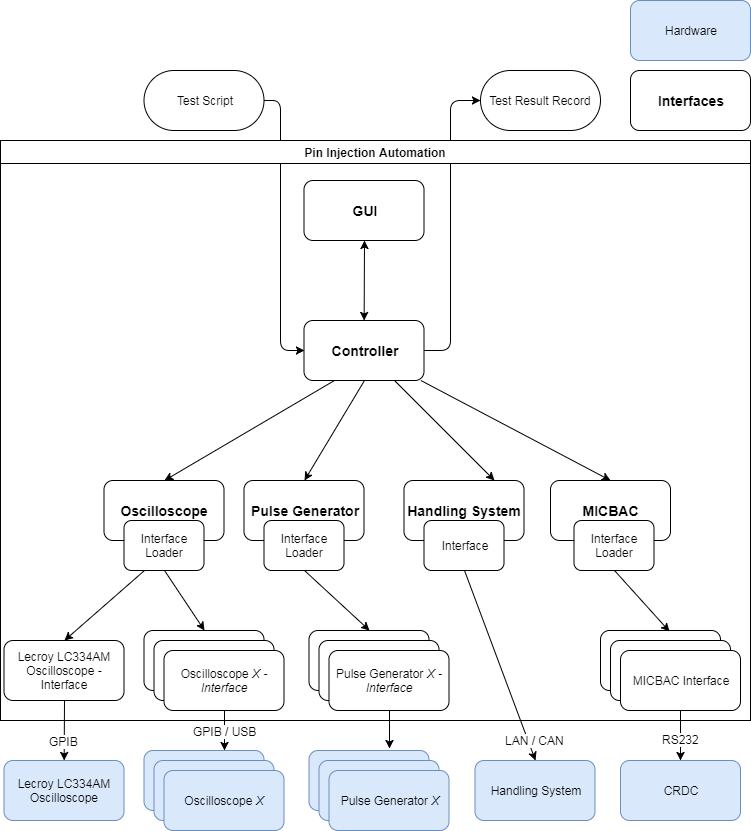
\includegraphics[width=0.75\textwidth, height=0.75\textwidth]{graphics/program_architecture.png}
	\caption{Programm Architektur}
	\label{fig:prg_architecture}
\end{figure}

Abbildung \ref{fig:prg_architecture} zeigt die entwickelte abstrakte Programmstruktur,
welche im Programm auch umgesetzt und benutzt wurde. Dort sieht man auch, dass das Programm
mehrere Interfaces für Oszilloskope und Puls-Generatoren ansteuert. Diese Anforderung wurde am
Ende so implementiert, dass sofern irgendeine neue Hardware Komponente eingebettet werden soll,
nur kleine Teile wie \ac{zb} die Auswahlmöglichkeit in der \ac{gui} erweitert werden muss. Die
eigentliche Programmstruktur wird dadurch nicht verändert, was die Flexibilität erhöht und es
so möglich ist das Programm nur durch hinzufügen einer neuen Datei, unter der Einhaltung von
einer bestimmten  Namensvergebung, zu erweitern. Erkennbar ist auch, dass die Aufgaben in
unterschiedliche Interfaces unterteilt wurden, was die Programmübersicht erhöht und  interne
Abhängigkeiten verringert. Dadurch sind \ac{zb} teile der \ac{gui} des öfteren ohne großen
aufwand schnell austauschbar gewesen, was mir im Verlaufe des Praktikums öfters mal sehr viel
Zeit eingespart hat.

	
\subsection{Python 3 als Programmiersprache}
\label{subsec:py3_as_lang}

Wie schon in Kapitel \ref{sec:prj-einarbeitung} erwähnt war es mir frei zu wählen, in welcher
Programmiersprache ich das Projekt realisieren möchte. Meine Entscheidung fiel dabei schnell
auf \citefield{Python}{note} 3, da auch die Erfahrung mit dieser Sprache auf der Seite des 
Kunden sehr groß war. Den Vorteil in dieser Sprache sehe ich darin, dass \citefield{Python}
{note} eine sehr aktuelle und dynamische Programmiersprache ist, welche sich schnell 
weiterentwickelt. 

Das Hauptmerkmal von \citefield{Python}{note} ist die Lesbarkeit und wird durch Code Style 
Richtlinien und Idiome realisiert. Diese Lesbarkeit wird auch \textit{Pythonic Way} genannt. 
Die Idiome in \citefield{Python}{note} lassen zukünftige Leser genau verstehen, was der Code 
machen soll, während die Code Style Richtlinien für einen einheitlichen Code sorgen.

Die Softwareanforderung wie \ac{zb} Datensätze aus einer \ac{csv} Datei auszulesen und zu 
verarbeiten konnte mit Hilfe der von \citefield{Python}{note} zur Verfügung gestellten \ac{api} 
sehr schnell realisiert werden. Des weiteren standen \citefield{Python}{note} Module für das 
Verarbeiten von \ac{micbac} Kommandos aus einem vorherigen Projekt bereits zur Verfügung.


\section{Die Erste Simulation}
\label{sec:first_simulation}

Die erste Aufgabe am Projekt war das erstellen einer Simulation. Die Simulation sollte am 
Anfang nur die Architektur implementieren und die Ausgabe für den Benutzer simulieren. Im 
Verlaufe des Praktikums wurden dann diese Ausgaben mit echten Werten verknüpft.

Um zu garantieren, dass die Softwarequalität bestehen bleibt, habe ich auf dem interen GitLab
\footnote{\url{https://about.gitlab.com/}} Server von Konzept einen sogenannten GitLab Runner
\footnote{\url{https://docs.gitlab.com/runner/}} erstellt. Dieser prüft den Codestyle von Python, läuft Tests durch und analysiert den Code.


\subsection{Konfigurieren des GitLab Runner}
\label{subsec:gitlab_runner}

Um den Runner nicht jedes mal beim einchecken neu aufbauen zu müssen und die Daten immer mit 
den selben Eigenschaften eingecheckt werden, habe ich ein \citefield{Docker}{note} Image, ein 
Speicherabbild eines Containers, erstellt.

\citefield{Docker}{note} wird zur Isolierung von Anwendungen mit Containervirtualisierung 
genutzt. Diese Container gewährleisten die Trennung und Verwaltung der auf dem Rechner 
genutzten Ressourcen und vereinfacht die Bereitstellung von Anwendungen, weil sich die 
Container leicht als Dateien transportieren und installieren lassen.

\begin{figure}[H]
	\centering
	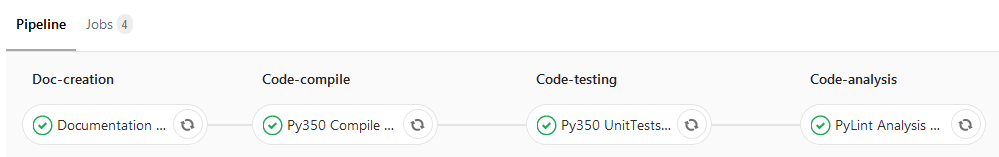
\includegraphics[width=1\textwidth, height=0.2\textwidth]{graphics/pipeline.png}
	\caption{Konfigurierte Pipeline}
	\label{fig:pipeline}
\end{figure}

In Abbildung \ref{fig:pipeline} stellt die Pipeline die Schritte dar, die durchlaufen werden.
Dazu gehört die Erstellung einer \ac{api} aus den Python Doc-Strings, die Code Kompilierung, 
das durchlaufen der Unit Tests und das durchlaufen von \citefield{Pylint}{note}. 
\citefield{Pylint}{note} ist ein statisches Codeanalyse Tool, das unter anderem den Code auf 
die Einhaltung der in \citefield{PEP8}{note} beschriebenen Regeln prüft.


\subsection{Einlesen von CSV-Dateien}
\label{subsec:read_csv}

Ein großer Bestandteil des Programms waren die eingelesenen Daten, welche in einem \ac{csv}-
Dateiformat abgespeichert wurden. Diese Aufgabe habe ich mittels der Klasse \textit{DictReader} 
gelöst, welche in der \citefield{Python}{note} \ac{api} vorhanden ist. Diese Klasse liest jede 
Zeile der \ac{csv}-Datei in ein \textit{Dictionary} \ac{bzw} den Python Datentyp \textit{dict} 
ein. Ein \textit{Dictionary} ist eine unsortierte, veränderbare und indexierte Kollektion aus 
\textit{Key-Value-Paaren}. Die Klasse \textit{DictReader} nimmt die erste Zeile der \ac{csv}-
Datei als \textit{Keys} und fügt die restlichen Zeilen als \textit{Values} ein. 
Da der Reader beim einlesen von Daten sehr sensibel ist und bei einem falschen Format \ac{bzw} 
bei falschen \textit{Key}-Werten oder auch bei falschen \textit{Value}-Werten direkt Fehler 
wirft, mussten diese irgendwie abgefangen und behandelt werden. Ein Problem war das erkennen 
und überspringen von Kommentaren. Kommentare haben in einer Datei immer mit dem \textit{\#}-
Zeichen angefangen. 

\inputpython{scripts/read_csv.py}{1}{14}{Read From CSV-File}{lst:read_csv}

In dem Code Listing \ref{lst:read_csv} sieht man eine Zusammenfassung des Codes, welcher für 
das Einlesen der Daten zuständig ist und die Python-private Methode \textit{skip\_comments()}, 
welche Kommentare erkennen und überspringen soll. Die Kommentare sollten möglichst bevor die 
Daten als Wert in ein \textit{Dictionary} gespeichert werden herausgefiltert werden. Dies habe 
ich mit einem \ac{regex} (engl: Regular Expression) gelöst, welcher die Zeile nach dem 
\textit{\#}-Zeichen absucht und falls eins gefunden wurde alle nachgehenden Zeichen inklusive 
dem \textit{\#}-Zeichen in der Zeile subtrahiert und die subtrahiert Zeile dann wieder 
zurückgibt.


\subsection{Erstellung einer GUI}
\label{subsec:create_gui}

Nachdem die Textuelle Simulation abgeschlossen war machte ich mich an die Erstellung einer 
\ac{gui}. Da vom Projekt keine Vorgaben existierten, konnte ich bei vielen selbst Entscheiden 
wie diese implementiert werden.
Die Abbildung \ref{fig:pipeline} zeigt die \ac{gui} mit dem Stand zum Ende des Praktikums. Die Tabelle, welche die Zeilen anzeigt, kann den gerade laufenden Test 
markieren, anzeigen ob die vorherigen Tests erfolgreich durchgelaufen sind oder nicht, einzelne 
Zeilen zum Testen auswählen und die Zeilen nach einer bestimmten Spalte sortieren. 
Die Tabelle wurde als virtuelle Tabelle implementiert. Das bedeutet, dass die Tabelle mit Hilfe 
der eingelesenen \ac{csv}-Datei indirekt adressiert wird und die Realisierung nicht direkt 
angesprochen wird. Damit war es sogar möglich eine \ac{csv}-Datei mit über 1 Millionen Zeilen 
innerhalb von ca. 20-30 Sekunden einzulesen und anzuzeigen. Links von dieser Tabelle habe ich einen sogenannten Verzeichnisbaum implementiert der die Verzeichnisstruktur von einem frei wählbaren Ordner aufbaut und anzeigt. Der Baum arbeitet viel mit Rekursion, denn er lädt nicht alle Strukturen der Unterverzeichnisse, sondern nur die erste \ac{bzw} die zu sehende Ebene. Damit die zu sehende Ebene richtig generiert wird muss beim laden geprüft werden ob der Pfad ein Ordner ist oder eine Datei. Ist der Pfad eine Datei so muss nichts weiter geprüft werden. Ist der Pfad aber ein Ordner, so muss überprüft werden ob dieser Ordner Dateien enthält oder nicht. Würde dies nicht geprüft werden, so wäre es nicht möglich über den Baum der \ac{gui} zugriff auf die Unterordner zu bekommen. Des weiteren ist der Baum so implementiert dass sobald der Fokus wieder auf die \ac{gui} gerichtet wird der Baum alle generierten Ebenen auf gelöschte oder neu hinzugefügte Dateien überprüft und nach generiert.

\begin{figure}[H]
	\centering
	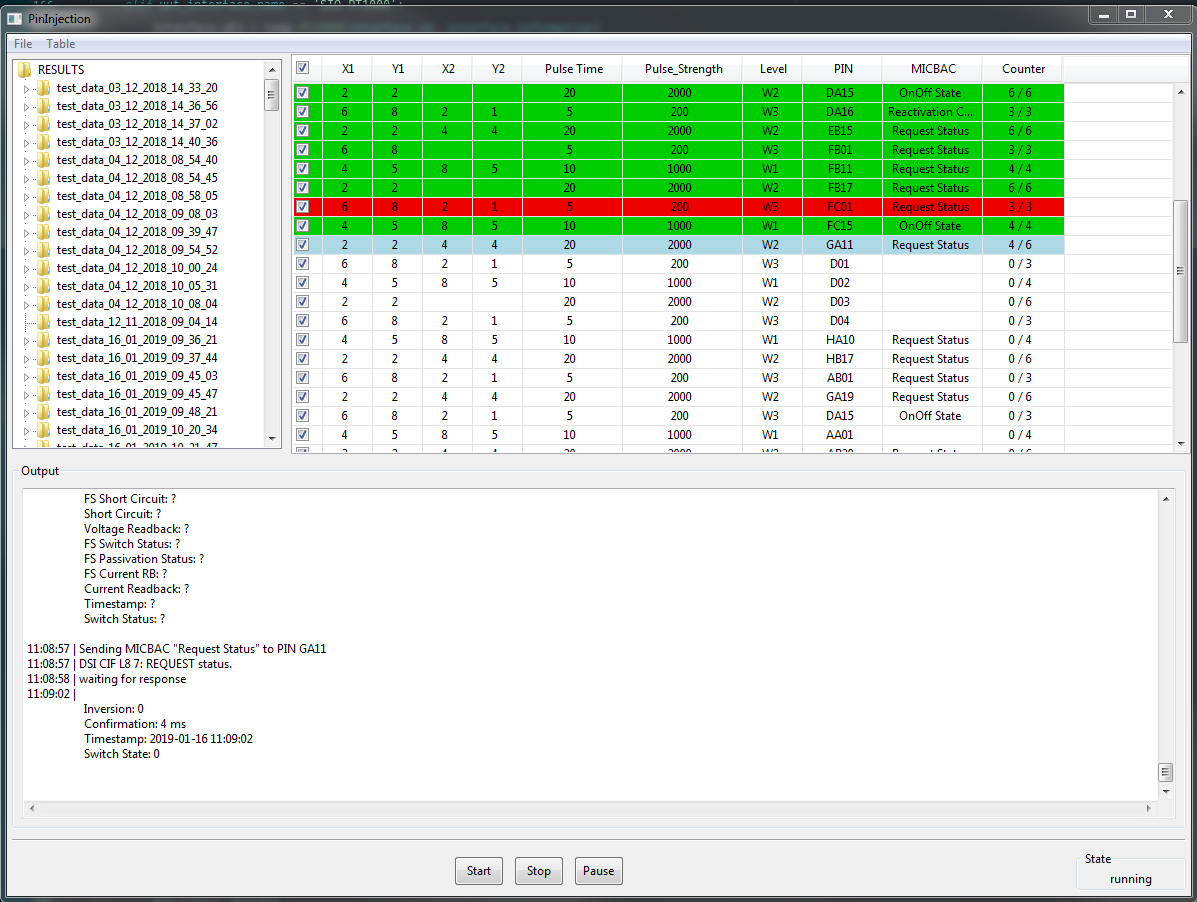
\includegraphics[width=1\textwidth, height=0.75\textwidth]{graphics/GUI.png}
	\caption{Graphical User Interface}
	\label{fig:pipeline}
\end{figure}


%+-----------+
%| Kapitel 2 |
%+-----------+
\chapter{Ansteuerung des Oszilloskop}
\label{ch:osci}

Im weiteren Verlauf meines Praktikums wurde mir irgendwann die Ansteuerung und die Implementierung eines Oszilloskopes zu Teil. 
Abbildung \ref{fig:lc334am} zeigt das Lecroy LC334AM 500Mhz Oszilloskop, welches über die \ac{gpib} Schnittstelle mit dem Computer kommunizieren kann. Der \ac{gpib} von \ac{ni}\footnote{\url{http://www.ni.com/de-de.html}} ist ein Industriestandard, welcher als \ac{ieee}\footnote{\url{https://www.ieee.org/}} veröffentlicht wurde.

\begin{figure}[H]
	\centering
	\includegraphics[width=0.75\textwidth, height=0.5\textwidth]{graphics/Programmed_Oscilloscope.png}
	\caption{Lecroy LC334AM 500MHz}
	\label{fig:lc334am}
\end{figure}




%+-----------+
%| Kapitel 3 |
%+-----------+
\chapter{Ansteuerung eines RDC}
\label{ch:micbac}


\begin{figure}[H]
	\begin{minipage}{0.5\textwidth}
		\centering
		\includegraphics[width=\textwidth, height=0.5\textwidth]{graphics/crdc_1.png}
		\caption{CRDC Type A Pins}
		\label{fig:crdc-pins}
	\end{minipage}
	\begin{minipage}{0.5\textwidth}
		\centering
		\includegraphics[width=\textwidth, height=0.5\textwidth]{graphics/crdc_2.png}
		\caption{CRDC Type A}
		\label{fig:crdc_top}
	\end{minipage}
\end{figure}



footnote und etc

\section{Verbindung herstellen über das RS232-Interface}
\label{sec:rs232-connection}

mach sachen

\section{Befehle Senden und Empfangen}
\label{sec:com-send-receive}

\subsection{MICBAC Commands}
\label{subsec:micbac-commands}

\subsection{Senden von MICBAC Commands}
\label{subsec:send-micbac}


\inputpython{scripts/send_micbac.py}{1}{15}{Send MICBAC Command}{lst:send-micbac}

\subsection{Empfangen von MICBAC Commands}
\label{subsec:receive-micbac}

\inputpython{scripts/receive_micbac.py}{1}{9}{Receive MICBAC Command}{lst:receive-micbac}

%+-----------+
%|   Fazit   |
%+-----------+
\chapter{Fazit}
\label{ch:fazit}

Während meiner Tätigkeit bei Konzept Informationssysteme traf ich auf vielseitige Aufgaben, 
die oftmals mit vielen Problemen verknüpft waren. Durch das Anwenden von angeeigneten 
Kenntnissen im Rahmen meines Studiums, die Chance eigene Ideen mit einfließen zulassen und 
verschiedenste Herangehensweisen auszuprobieren verhalfen mir meist diese Probleme zu 
lösen. Manchmal stieß ich auf Herausforderungen wie \ac{zb} die Verarbeitung empfangener 
Daten vom LC334AM Oszilloskop, die ich nur durch alleiniges aneignen und verbinden von 
oftmals schwer zu findenden Informationen überwinden konnte.

Durch den Einstieg in ein komplett neu angenommenes Kundenprojekt hatte ich Einblick in 
viele Phasen der Umsetzung. Dazu zählte das Mitwirken bei Entwicklung und Gestaltung des 
Programmes, Wünsche und Anforderungen vom Kunden in Form von Meetings zu besprechen und ins 
Programm zu integrieren, sowie die Ausarbeitung von Lösungen verschiedenster auftretender 
Herausforderungen.

Mit diesen Einblicken konnte ich mich sowohl fachspezifisch, fächerübergreifend als auch 
persönlich weiterbilden und durch die vielen gesammelten Erfahrungen weiterentwickeln. 
Besonders mein Interesse im Bereich Embedded Systems hat sich nochmals gestärkt. Meine 
Fachkenntnisse, insbesondere Python, konnte ich in vielen Bereichen vertiefen. Weiterhin 
erlangte ich einen Blick auf den Firmenalltag, Abläufe und Veranstaltungen wie \ac{zb} das 
Präsentieren der Firma bei der Firmenmesse in der Hochschule Ravensburg-Weingarten
\footnote{\url{https://www.hs-weingarten.de/web/willkommen/startseite}} oder auch interne 
Veranstaltungen wie \ac{zb} den Jahresabschluss, der im Schloss Tettnang abgehalten wurde.

Die besonders freundlichen Kollegen sowie das mir zugeteilte Projekt selbst prägten mein 
Praktikum sehr positiv. Durch die Hilfe der Kollegen sowie das freundschaftliche 
miteinander sorgten dafür das es mir während der Arbeit an nichts mangelte. Gesten wie 
\ac{zb} das mitbringen von selbstgebackenen Kuchen von meinem Projektleiter erfreute meine 
Kollegen und mich jedes mal aufs neue. Abschließend kann ich ein Praxissemester bei Konzept 
absolut empfehlen.

%+----------------------+
%| Abkürzungsverzeichnis|
%+----------------------+
\section*{Abkürzungsverzeichnis}
\begin{acronym}[MICBAC]
\acro{api}[API]{Application Programming Interface}
\acro{bsp}[bsp.]{Beispiel}
\acro{bzw}[bzw.]{beziehungsweise}
\acro{csv}[csv]{Comma-separated values}
\acro{gpib}[GPIB]{General Purpose Interface Bus}
\acro{gui}[GUI]{Graphical User Interface}
\acro{ieee}[IEEE 488]{Institute of Electrical and Electronic Engineers Standard 488}
\acro{micbac}[MICBAC]{Micro System Bus Access Channel}
\acro{ni}[NI]{National Instruments}
\acro{pia}[PiA]{Pin-Injection Automation}
\acro{regex}[regex]{Regulärer Ausdruck}
\acro{rs232}[RS-232]{Recommended Standard 232}
\acro{zb}[z.B.]{zum Beispiel}
\end{acronym}

%+--------------------------+
%| Ehrenwörtliche Erklärung |
%+--------------------------+
\pagenumbering{gobble}
\chapter*{Ehrenwörtliche Erklärung}

Hiermit erkläre ich, dass ich den vorliegenden Bericht selbstständig 
angefertigt und alle von mir genutzten Quellen und Hilfsmittel angegeben 
habe. Dieser Bericht wurde bisher in keiner anderen Prüfungsbehörde oder 
Person im Rahmen einer Prüfung vorgelegt und auch nicht veröffentlicht.

\vspace{5cm}

\rule{3.5cm}{1pt} \hspace{1.5cm} \rule{10cm}{1pt}\\
Datum \hspace{4cm} Unterschrift\\



%+==============+
%| DOCUMENT END |
%+==============+
\end{document}

